% ---------------------------------------------------------------------------
% ACT D (MULTIPOINT OPTIMISATION) -- ONE SHAPE, THREE ANGLES OF ATTACK.
% One-page customer-facing result sheet for the A1 NACA0012 alpha-multipoint
% SHAPE OPTIMISATION.  Compile: pdflatex ACT_D_multipoint_optimisation_sheet.tex
%
% RELATION TO THE OTHER TWO ACT D SHEETS IN THIS DIRECTORY.  Three different
% subjects have been called "Act D" and their numbers must never be merged:
%   ACT_D_aerofoil_section_sheet.tex   2D NACA0012, SO-3aR2 run root, gradients
%                                      verified at the BASELINE, NO OPTIMISER RAN.
%   ACT_D_reference_wing_sheet.tex     3D reference wing, 38,304 cells, 47 majors.
%   THIS SHEET                         2D NACA0012, 4,032 cells, SO-3 run root,
%                                      the OPTIMISER RAN and the gradient is
%                                      verified AT THE FINAL DESIGN POINT.
% This sheet supersedes NOTHING.  It is the successor rung to the first of them.
%
% ---------------------------------------------------------------------------
% WHICH ROW IS ON CAMERA, AND WHY (not rendered).
% The item graded TWO rows, SHIPPED and PATCHED, on two builds of the mesh
% deformation library.  Both rows are PASS.  THIS SHEET CARRIES THE PATCHED ROW
% ONLY, because a demo shows ONE run and which library build produced it is
% METHOD, which the demo may withhold.  It may never misstate a RESULT, and it
% does not: every number below is the PATCHED row's own.
% THE TWO ROWS ARE NOT PRESENTED AS A REPEATABILITY PAIR AND MUST NOT BE.  Their
% gradient components diverge by up to 24.17 % (grade JSON,
% divergence_shipped_vs_patched.worst_pct), so quoting them as run-to-run
% reproduction would overstate by more than two orders of magnitude.
%
% BUT THE FACE NOW STATES THAT BOTH ROWS RAN AND BOTH PASSED, because the
% two-row rule is a rule about the VERDICT, not about the camera: a DAFoam
% verdict is two rows, shipped and patched, or it is not a verdict about
% DAFoam.  The Table 4 row `Runs of this case, both inside the limit  2 of 2`
% and the three-sentence note under it carry that fact WITHOUT pairing the two
% runs and WITHOUT putting the second design on screen.  Measured basis, grade
% JSON: verdict PASS; rows {"SHIPPED": "PASS", "PATCHED": "PASS"}; gates.G5J
% <ROW>.G5J_objective.worst_rel_err_pct = 0.18905998172513677 SHIPPED and
% 0.2533162674763216 PATCHED, both against band_D_pct = band_E_pct = 5.0, each
% 4 of 4 pairs, n_gate_fail 0.  The note says in terms that the two runs do not
% return the same shape and are not a repeat of one another, so no reader can
% take the two percentages as an agreement pair.  No verdict token, no row
% name, no library-build name reaches the rendered face.
%
% ---------------------------------------------------------------------------
% PROVENANCE OF EVERY USER-VISIBLE NUMBER (not rendered; for the lab only).
% Run root:
%   /home/ubuntu/certonomous-runs/
%     CURRICULUM-SO3-a1-naca0012-alpha-multipoint-optimisation/
% Frozen grade file (item verdict PASS, rows SHIPPED PASS / PATCHED PASS):
%   SO3_grade_20260901T040709Z.json
% Chain: STATUS.chain, `chain=COMPLETE declared=7 executed=7`, all seven arms rc=0.
% Extracted, with a planted reader control, into:
%   cases/dafoam/ladder-a/A1_so3_demo_series.json
%   by cases/dafoam/build_so3_demo_series.py
%
%   TABLE 1 operating condition
%     U0=10, p0=0, nu=1.5e-5, A0=0.1, rho0=1.0, chord 1 m:
%       O-P/so3_runScript.py lines 221-231, 299-309;
%       O-P/constant/transportProperties (`nu 1.5e-5`)
%     turbulence model SpalartAllmaras: O-P/constant/turbulenceProperties
%     solver DASimpleFoam: O-P/so3_runScript.py:286
%     alphas and weights, registered 3.13918623195176 / 5.13918623195176 /
%       7.13918623195176 and 1/3 each, tolerance 1e-12, read back with
%       abs_deviation 0.0 on all four artefacts:
%       grade JSON gates.G-ALPHA_operating_points (verdict PASS)
%     mesh 4032 cells: grade JSON mesh_cells, and counted independently by
%       cases/dafoam/render_so3_mesh_figures.py off the front symmetry patch
%       of MESH/constant/polyMesh (4032 faces in plan; the script REFUSES on
%       disagreement with the grade)
%     first layer height 2.0629e-03 to 4.0659e-03 m over 126 wall nodes:
%       measured by the same script off MESH/constant/polyMesh
%     far field radius 18.583 m about the grid centre (0.679, 0.000), with the
%       outermost nodes spanning 18.559 to 18.583 m, so the outer boundary IS a
%       circle and the figure is a radius.  max|x| reads 18.73 and is NOT the
%       radius; the earlier draft of this sheet quoted that and was corrected.
%     wall treatment nutUSpaldingWallFunction: O-P/0/nut, patch "(wing.*)"
%     8 shape design variables, bounds +/-1.0; thickness in [0.5, 3.0], volume
%       >= 1.0, leading-edge radius >= 0.8:
%       O-P/so3_runScript.py lines 448, 457-459
%     FFD stations x = -0.010, 0.245, 0.500, 0.755, 1.010 and y = +/-0.07,
%       block 5x2x2: O-P/FFD/wingFFD.xyz (read directly)
%
%   TABLE 2 result, PATCHED row, from grade JSON
%   gates.G-OPT9_optimisation_per_row.PATCHED:
%     CD_baseline [0.01723938072177922, 0.020910510045267394,
%                  0.027268054119716875]
%     CD_final    [0.016254689517250072, 0.017469887014380677,
%                  0.02112501252302095]
%     CL_baseline [0.31189588769251864, 0.49876526085592926,
%                  0.6639763551107052]
%     CL_final    [-0.05675565457564216, 0.15320276361213012,
%                  0.3611940124520788]
%     J_baseline  0.02180598162892116   J_final 0.018283196351550565
%     weighted_drag_reduction_pct 16.15513273980908
%   THAT PERCENTAGE IS QUOTED ONLY IN A TABLE THAT ALSO CARRIES CL_baseline AND
%   CL_final, BECAUSE THE GRADE FILE'S OWN forbidden_readings FORBID QUOTING IT
%   OTHERWISE: "quoting the weighted-drag reduction without CL_baseline and
%   CL_final beside it, because CL is UNCONSTRAINED in this item".
%   The endpoint arm's own CL_baseline field (XE-P/so3_X.json) reads
%   [-0.05675568..., 0.15320274..., 0.36119399...], i.e. the FINAL design
%   point, and corroborates the CL_final row above to 7 significant figures.
%
%   TABLE 3 optimiser, from the same gate block and from the IPOPT table in
%   O-P_20260901T035101Z_1094485.log parsed by the frozen so3_stall.parse_majors:
%     optimiser IPOPT; n_majors 10 (this reader and the frozen grader agree, and
%       build_so3_demo_series.py REFUSES if they do not); max_iter_registered 50;
%       tol_registered 1e-05; exit "Optimal Solution Found.";
%       cumulative_line_search_cutbacks 0; n_restoration_majors 0;
%       last_inf_du 7.28e-06; stall "NO_STALL"
%     objective per major, iterations 0 to 9:
%       0.021805981 0.021758387 0.019453909 0.018604447 0.018430271
%       0.018327450 0.018303722 0.018284843 0.018283942 0.018283197
%
%   TABLE 4 and FIGURE 4, endpoint gradient check, PATCHED row, from grade JSON
%   gates.G5J.PATCHED.G5J_objective (verdict PASS, 4 of 4 pairs, band 5.0 %,
%   plateau tolerance 10 %, steps [1e-2, 1e-3, 1e-4], reference step 1e-3):
%     shape[0] adjoint -0.00558919054767835  fd -0.00558114277299758  0.1442 %
%     shape[3] adjoint  0.0045540908755884926 fd 0.00455796217...     0.0849 %
%     shape[6] adjoint -0.015521078767334174 fd -0.0155274194...      0.0408 %
%     shape[7] adjoint -0.0018004479396249767 fd -0.00179589864...    0.2533 %
%     worst 0.2533162674763216, aggregate 0.06890419283803313
%   Control-name map, derived from O-P/FFD/wingFFD.xyz and the shape-function
%   construction at O-P/so3_runScript.py:409-422 (5x2x2 FFD: interior i=1,2,3
%   with j=0 lower / j=1 upper give indices 0..5 in that order; i=0 and i=4 give
%   the two symmetric edge pairs as indices 6 and 7):
%     shape[0] lower surface at x/c = 0.245   shape[3] upper surface at x/c = 0.500
%     shape[6] leading-edge pair              shape[7] trailing-edge pair
%   The gate stands at the FINAL design point, not the baseline: grade JSON
%   gates.G-DESIGNPOINT..., design_point "FINAL" on all four artefacts, xopt
%   sha256 ccc1bb80... pinned per PATCHED row, verdict PASS.
%
%   TABLE 5 instrument checks, from grade JSON `controls`:
%     grader_plant_X_PATCHED: plant 0.0008371714159496371 sized at
%       3.0*(5.0/100)*|d_ref|, planted_rel_err_pct 15.0, seen True, and the
%       gate MOVED under it: G5J_unplanted PASS -> G5J_planted GATE FAIL, and
%       g_mp_struct_unplanted PASS -> g_mp_struct_planted GATE FAIL
%     grader_plant_F_PATCHED: seen True over 112 values, worst residual
%       1.7932703932910243e-16
%     grader_plant_cells: on_disk_before_plant 4032, want 4039, read_back 4039
%     instrument_ctrl_PATCHED: seven quantities, want 0.617, read 0.617 on all
%       seven, both_directions True
%     G_TB_trivial_baseline PATCHED: at a deliberately unsuitable step, 0 of 4
%       components pass the band (max allowed 1); worst 107.89 %, best 73.45 %
%     G_MP_STRUCT_assembly_identity PATCHED: worst relative residual
%       8.864158539519277e-14 against a 1e-10 tolerance, 4 of 4 components PASS
%     grader_plant_c5: on the O-S log, 6842 real lines, 1 positive site,
%       0 negative sites, seen True
%
%   TABLE 6 compute, PATCHED path only (MESH + O-P + XE-P + FE-P), from grade
%   JSON gates.G10_caps.per_arm and the run root's ledger.txt ARM= rows:
%     MESH  predicted 0.19  actual 0.167 core-min (10 wall s)  ratio 0.8789
%     O-P   predicted 103.0 actual 6.950 core-min (417 wall s) ratio 0.0675
%     XE-P  predicted 3.7   actual 2.533 core-min (152 wall s) ratio 0.6846
%     FE-P  predicted 7.5   actual 4.533 core-min (272 wall s) ratio 0.6044
%     path totals: predicted 114.39, actual 14.183 core-min, 851 wall s, 0.124
%   THE PREDICTED COLUMN IS OFF THE RENDERED FACE AND THE ACTUALS ARE NOT.
%   Table 6 shows measured core-minutes and measured wall seconds only.  A
%   PREDICTION MUST NEVER STAND ON CAMERA AS WHAT THE RUN COST, and 114.39 is a
%   prediction twice over: it is a lane's sum of four per-arm `predicted`
%   fields, and this item's own registered cost prediction (P_COST, point
%   228.59 core-min, band [60, 300]) scored MISS against a measured 28.900
%   core-min for the whole item -- out by nearly a factor of eight.  The
%   estimate-versus-actual comparison rule 12 requires is not lost: it is filed
%   as this item's row in docs/COST_CALIBRATION.md at ratio 0.126, and the
%   per-arm predicteds and ratios stay in this block above.
%   Wall seconds on the face are the same arms' clocks: 10 + 417 + 152 + 272 =
%   851 s, and ranks=1 throughout, so each core-min figure is that arm's wall
%   seconds over sixty.
%     dollars 14.183/60*0.0513 = 0.012127 -> $0.0121 DERIVED, NOT MEASURED
%     (c7a.4xlarge at $0.0513/core-h, REPORTED-BY-OWNER; the box cannot read its
%     own billing).  ranks=1 on every arm, so core-min = wall s / 60 exactly.
%   The whole seven-arm item cost 28.900 core-min / $0.02471 against a 595.0
%   ceiling with no arm crossing its cap (grade JSON gates.G10_caps, verdict
%   PASS); that item-level figure is in the calibration ledger, not on camera,
%   because this sheet shows one run.
%
%   ASSUMED, NOT MEASURED, and kept out of every measured table:
%     speed of sound 340 m/s (standard sea-level air) for the Mach row
%     y+ about 30 to 60, estimated as u_tau*y/nu with y the half of the measured
%       first layer height and cf = 0.026 Re^(-1/7) (flat-plate correlation):
%       cf = 0.00383, u_tau = 0.438 m/s, y = 1.03e-3 to 2.03e-3 m.
%       THE RUN WRITES NO y+ FIELD, so this is a correlation, never a reading.
%
% ---------------------------------------------------------------------------
% BINDING CAPTURES THIS SHEET IS WRITTEN TO (not rendered).
%   Act A figure and header standard, applies to every act: header carries the
%   solver line of the source run; figures carry no paragraphs; title at most
%   10 words; axis labels with units; legend inside the axes; one caption line
%   of at most 20 words; explanation moves to the sheet text; no meta-commentary
%   about the figure; sheet paragraphs at most 3 sentences.
%   Demo mode: every number, field and figure is the real run's; present-tense
%   solved-case wording; no replay, storage or substitution language anywhere.
%   Overnight order: live-looking, synchronized, no internal information, no
%   past tense, short sentences, all results in tables, real geometry and its
%   real mesh only, professional prompts, all plots latexified.
%   Standing product rules: repeated per-item numbers are always a table; every
%   plot self-explanatory; name the reference area for any coefficient; state
%   the finite-difference step AND that it was swept; y+ range and wall
%   treatment on the mesh table; measured and assumed never share a table
%   header; no dashes on a camera surface; no repository paths on camera.
%
%   ONE ITEM REFERRED UPWARD AND NOT DECIDED HERE.  A capture directs that the
%   dafoam demo show 20 minutes everywhere rather than 60.  It attaches to a
%   3601 s figure on the reference-wing act, not to this run.  This sheet shows
%   THIS run's measured 851 wall s, which is 14.2 minutes and therefore already
%   under twenty; no time figure here is invented and none contradicts that
%   instruction.  Whether the 20-minute display figure is meant to extend to
%   this act is not a lane's call and is referred.
% ---------------------------------------------------------------------------
\documentclass[9pt,a4paper]{article}
\usepackage[margin=8mm,top=5mm,bottom=2mm]{geometry}
\usepackage{booktabs}
\usepackage{array}
\usepackage{xcolor}
\usepackage{graphicx}
\usepackage{amssymb}
\usepackage[T1]{fontenc}

\definecolor{band}{rgb}{0.87,0.91,0.96}
\definecolor{accent}{rgb}{0.10,0.32,0.60}
\definecolor{warm}{rgb}{0.72,0.30,0.06}
\definecolor{rulegrey}{rgb}{0.45,0.45,0.45}
\definecolor{boxgrey}{rgb}{0.96,0.96,0.94}

\renewcommand{\footnotesize}{\fontsize{6.4}{6.85}\selectfont}
\renewcommand{\scriptsize}{\fontsize{5.7}{6.1}\selectfont}
\renewcommand{\arraystretch}{0.97}
\setlength{\parindent}{0pt}
\setlength{\parskip}{0pt}
\setlength{\tabcolsep}{3.2pt}
\pagestyle{empty}

\newcommand{\rolesig}[1]{\textbf{\footnotesize#1}}
\graphicspath{{../../../cases/dafoam/ladder-a/figures/}}

\begin{document}
% BODY LEADING 8.5 -> 8.0 (type size unchanged at 7.3pt).  The sheet is ONE
% page by standard and had no vertical slack: measured, a single extra table
% row alone pushed it to two.  The two-run statement and its table row need
% about 28pt, and every alternative was measured before this one was taken --
% column rebalancing, table stretch, top margin and the caption leadings each
% bought under 10pt.  At 7.3/8.0 the body is still looser than the sheet's own
% footnote and caption blocks (6.4/6.85 and 5.7/6.1).  No content is cut to
% make the room.
\fontsize{7.3}{8.0}\selectfont

% ---------------------------------------------------------------- title -----
{\fontsize{13.5}{15}\selectfont\bfseries One shape, three angles of attack}\\[1.5pt]
{\fontsize{8.6}{10}\selectfont Gradient driven shape optimisation of a
NACA0012 section, incompressible, steady, two dimensional}\\[2pt]
{\color{rulegrey}\rule{\textwidth}{0.9pt}}\\[1pt]
{\footnotesize \textbf{Solver: DAFoam \texttt{DASimpleFoam}, steady
incompressible RANS, Spalart-Allmaras turbulence, discrete adjoint, IPOPT.}
Your request: \emph{minimise the drag of this section averaged over three
angles of attack, $3.139$, $5.139$ and $7.139$ degrees, weighted equally, at
$10\,\mathrm{m\,s^{-1}}$; one shape serves all three; verify the gradient at
the final shape.}}

% ================================================================= row 1 =====
\vspace{2.5pt}
\begin{minipage}[t]{0.505\textwidth}
\textbf{What the optimiser does, and what it costs you}

\vspace{1pt}
{\footnotesize The weighted drag objective falls by $16.2$ per cent in ten
major iterations. The optimiser stops on its own tolerance, not on the
iteration cap. \textbf{Lift carries no constraint in this problem, and the
optimiser spends it}: every lift coefficient falls, and at the lowest angle
$C_L$ goes negative.\\[2pt]
\textbf{What this run establishes.} The gradient that drove the descent is
checked against an independent calculation \emph{at the final shape}, and agrees
to $0.25$ per cent at worst against a five per cent limit fixed beforehand. The
optimiser and the gradient are verified; the section is not a better aerofoil.}

\vspace{2.5pt}
\textbf{Table 1. Operating condition and grid.}

\vspace{1.5pt}
{\fontsize{6.7}{7.9}\selectfont
\begin{tabular}{@{}l r l l@{}}
\toprule
Quantity & Value & Unit & Basis \\
\midrule
Freestream speed $U$          & $10$                & m\,s$^{-1}$     & exact input \\
Chord $c$                     & $1$                 & m               & exact input \\
Reference area $A$            & $0.1$               & m$^2$           & exact input \\
Viscosity $\nu$ (kinematic)   & $1.5\times10^{-5}$  & m$^2$\,s$^{-1}$ & exact input \\
Reynolds number $Uc/\nu$      & $6.67\times10^{5}$  &                 & derived, exact \\
Mach number                   & $0.029$             &                 & derived \\
Angles $\alpha$               & $3.139$, $5.139$, $7.139$ & deg       & registered \\
Weights                       & $1/3$ each          &                 & registered \\
Deviation on both, read back  & $0$                 &                 & measured, $10^{-12}$ \\
\midrule
Grid                          & $4\,032$            & cells           & counted \\
Far field radius              & $18.6$              & m               & measured \\
First layer height            & $2.06$ to $4.07$    & $10^{-3}$ m     & measured \\
Shape controls                & $8$                 &                 & design variables \\
\bottomrule
\end{tabular}}

\vspace{1pt}
{\scriptsize The wall treatment is a continuous wall function, valid across the
whole near-wall range. Coefficients are formed on the reference area above.}
\end{minipage}\hfill
\begin{minipage}[t]{0.475\textwidth}
\textbf{Figure 1. The grid the section is solved on.}

\vspace{1.5pt}
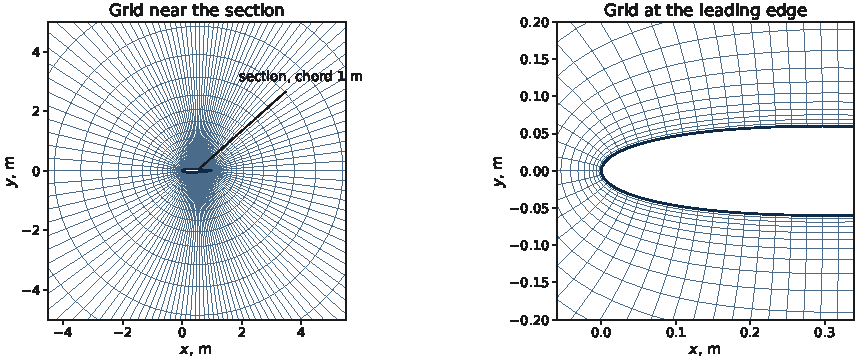
\includegraphics[width=0.90\textwidth]{so3_grid_pair.pdf}

\vspace{0.5pt}
{\scriptsize All $4\,032$ cells are drawn. The left view stops at about
$5\,\mathrm{m}$; the far field radius is $18.6\,\mathrm{m}$.}

\vspace{3pt}
\textbf{Table 2. The result. Drag and lift move together.}

\vspace{1.5pt}
{\fontsize{6.7}{7.9}\selectfont
\begin{tabular}{@{}r r r r r@{}}
\toprule
$\alpha$, deg & $C_D$ start & $C_D$ final & $C_L$ start & $C_L$ final \\
\midrule
$3.139$ & $0.017239$ & $0.016255$ & $0.31190$ & $\mathbf{-0.05676}$ \\
$5.139$ & $0.020911$ & $0.017470$ & $0.49877$ & $0.15320$ \\
$7.139$ & $0.027268$ & $0.021125$ & $0.66398$ & $0.36119$ \\
\midrule
Weighted $J$ & $0.0218060$ & $0.0182832$ & & \\
\bottomrule
\end{tabular}}

\vspace{1.5pt}
{\scriptsize $J$ is the equally weighted mean of the three drag coefficients and
it falls by $16.2$ per cent. Every lift coefficient falls with it, so the lift
columns are never quoted apart from the drag columns.}
\end{minipage}

% ================================================================= row 2 =====
\vspace{2pt}
{\color{rulegrey}\rule{\textwidth}{0.5pt}}\\[1pt]
\begin{minipage}[t]{0.50\textwidth}
\textbf{Figure 2. Drag and lift at three angles of attack.}

\vspace{2pt}
\setlength{\unitlength}{1mm}
\begin{picture}(75,30)(-6.5,-6.5)
  % ---------------- panel A: C_D -------------------------------------------
  \linethickness{0.4pt}
  \put(0,0){\line(1,0){27}}
  \put(0,0){\line(0,1){24}}
  \multiput(0,0)(0,9.2308){3}{\line(-1,0){1.1}}
  \put(-1.7,-0.8){\makebox(0,0)[r]{\scriptsize $0.015$}}
  \put(-1.7,8.4){\makebox(0,0)[r]{\scriptsize $0.020$}}
  \put(-1.7,17.7){\makebox(0,0)[r]{\scriptsize $0.025$}}
  \put(-5.6,12){\makebox(0,0)[c]{\rotatebox{90}{\scriptsize $C_D$}}}
  \multiput(6.279,0)(6.279,0){4}{\line(0,-1){1.1}}
  \put(6.279,-3.1){\makebox(0,0)[c]{\scriptsize $4$}}
  \put(12.558,-3.1){\makebox(0,0)[c]{\scriptsize $5$}}
  \put(18.837,-3.1){\makebox(0,0)[c]{\scriptsize $6$}}
  \put(25.116,-3.1){\makebox(0,0)[c]{\scriptsize $7$}}
  \put(13.5,-5.6){\makebox(0,0)[c]{\scriptsize $\alpha$, deg}}
  \linethickness{0.5pt}
  {\color{accent}\qbezier(0.874,4.134)(7.154,7.523)(13.434,10.912)
   \qbezier(13.434,10.912)(19.714,16.781)(25.994,22.649)
   \put(0.874,4.134){\circle*{1.1}}\put(13.434,10.912){\circle*{1.1}}
   \put(25.994,22.649){\circle*{1.1}}}
  {\color{warm}
   \multiput(0.874,2.316)(1.570,0.281){8}{\rule{0.9mm}{0.4pt}}
   \multiput(13.434,4.560)(1.570,0.844){8}{\rule{0.9mm}{0.4pt}}
   \put(0.174,1.616){\framebox(1.4,1.4){}}
   \put(12.734,3.860){\framebox(1.4,1.4){}}
   \put(25.294,10.608){\framebox(1.4,1.4){}}}
  \put(1.8,22.3){\makebox(0,0)[l]{\scriptsize\color{accent}$\bullet$\ start}}
  \put(1.8,19.6){\makebox(0,0)[l]{\scriptsize\color{warm}$\square$\ final}}
  % ---------------- panel B: C_L -------------------------------------------
  \put(41,0){
    \linethickness{0.4pt}
    \put(0,0){\line(1,0){27}}
    \put(0,0){\line(0,1){24}}
    {\color{rulegrey}\multiput(0,3)(3,0){9}{\rule{1.7mm}{0.3pt}}}
    \multiput(0,3)(0,6){4}{\line(-1,0){1.1}}
    \put(-1.7,2.2){\makebox(0,0)[r]{\scriptsize $0.0$}}
    \put(-1.7,8.2){\makebox(0,0)[r]{\scriptsize $0.2$}}
    \put(-1.7,14.2){\makebox(0,0)[r]{\scriptsize $0.4$}}
    \put(-1.7,20.2){\makebox(0,0)[r]{\scriptsize $0.6$}}
    \put(-5.2,12){\makebox(0,0)[c]{\rotatebox{90}{\scriptsize $C_L$}}}
    \multiput(6.279,0)(6.279,0){4}{\line(0,-1){1.1}}
    \put(6.279,-3.1){\makebox(0,0)[c]{\scriptsize $4$}}
    \put(12.558,-3.1){\makebox(0,0)[c]{\scriptsize $5$}}
    \put(18.837,-3.1){\makebox(0,0)[c]{\scriptsize $6$}}
    \put(25.116,-3.1){\makebox(0,0)[c]{\scriptsize $7$}}
    \put(13.5,-5.6){\makebox(0,0)[c]{\scriptsize $\alpha$, deg}}
    \linethickness{0.5pt}
    {\color{accent}\qbezier(0.874,12.357)(7.154,15.160)(13.434,17.963)
     \qbezier(13.434,17.963)(19.714,20.441)(25.994,22.919)
     \put(0.874,12.357){\circle*{1.1}}\put(13.434,17.963){\circle*{1.1}}
     \put(25.994,22.919){\circle*{1.1}}}
    {\color{warm}
     \multiput(0.874,1.297)(1.570,0.787){8}{\rule{0.9mm}{0.4pt}}
     \multiput(13.434,7.596)(1.570,0.780){8}{\rule{0.9mm}{0.4pt}}
     \put(0.174,0.597){\framebox(1.4,1.4){}}
     \put(12.734,6.896){\framebox(1.4,1.4){}}
     \put(25.294,13.136){\framebox(1.4,1.4){}}}
    \put(15.3,4.6){\makebox(0,0)[l]{\scriptsize\color{accent}$\bullet$\ start}}
    \put(15.3,1.9){\makebox(0,0)[l]{\scriptsize\color{warm}$\square$\ final}}
  }
\end{picture}

\vspace{1pt}
{\scriptsize Drag falls at every angle. Lift falls at every angle and turns
negative at the lowest.}

\vspace{3pt}
\textbf{Table 3. The optimiser.}

\vspace{1.5pt}
{\fontsize{6.7}{7.9}\selectfont
\begin{tabular}{@{}l r@{}}
\toprule
Quantity & Value \\
\midrule
Optimiser                               & IPOPT \\
Major iterations taken                  & $10$ \\
Iteration cap, fixed beforehand         & $50$ \\
Convergence tolerance, fixed beforehand & $1\times10^{-5}$ \\
Terminal statement                      & Optimal Solution Found. \\
Line search cutbacks                    & $0$ \\
Restoration iterations                  & $0$ \\
Dual infeasibility at the last major    & $7.28\times10^{-6}$ \\
\bottomrule
\end{tabular}}

\vspace{1pt}
{\scriptsize The optimiser prints its own convergence statement against its own
tolerance. It stops one fifth of the way into the iteration budget.}
\end{minipage}\hfill
\begin{minipage}[t]{0.475\textwidth}
\textbf{Figure 3. Objective against major iteration.}

\vspace{2pt}
\setlength{\unitlength}{1mm}
\begin{picture}(54,29)(-12,-6.5)
  \linethickness{0.4pt}
  \put(0,0){\line(1,0){40}}
  \put(0,0){\line(0,1){22}}
  \multiput(0,0)(0,5.5){5}{\line(-1,0){1.1}}
  \put(-1.7,-0.8){\makebox(0,0)[r]{\scriptsize $0.0180$}}
  \put(-1.7,4.7){\makebox(0,0)[r]{\scriptsize $0.0190$}}
  \put(-1.7,10.2){\makebox(0,0)[r]{\scriptsize $0.0200$}}
  \put(-1.7,15.7){\makebox(0,0)[r]{\scriptsize $0.0210$}}
  \put(-1.7,21.2){\makebox(0,0)[r]{\scriptsize $0.0220$}}
  \put(-10.6,11){\makebox(0,0)[c]{\rotatebox{90}{\scriptsize $J$}}}
  \multiput(0,0)(13.333,0){4}{\line(0,-1){1.1}}
  \put(0,-3.1){\makebox(0,0)[c]{\scriptsize $0$}}
  \put(13.333,-3.1){\makebox(0,0)[c]{\scriptsize $3$}}
  \put(26.667,-3.1){\makebox(0,0)[c]{\scriptsize $6$}}
  \put(40,-3.1){\makebox(0,0)[c]{\scriptsize $9$}}
  \put(20,-5.6){\makebox(0,0)[c]{\scriptsize major iteration}}
  \linethickness{0.5pt}
  {\color{accent}
   \qbezier(0.000,20.933)(2.222,20.802)(4.444,20.671)
   \qbezier(4.444,20.671)(6.667,14.334)(8.889,7.997)
   \qbezier(8.889,7.997)(11.111,5.661)(13.333,3.324)
   \qbezier(13.333,3.324)(15.556,2.846)(17.778,2.367)
   \qbezier(17.778,2.367)(20.000,2.084)(22.222,1.801)
   \qbezier(22.222,1.801)(24.444,1.736)(26.667,1.670)
   \qbezier(26.667,1.670)(28.889,1.619)(31.111,1.567)
   \qbezier(31.111,1.567)(33.333,1.565)(35.556,1.562)
   \qbezier(35.556,1.562)(37.778,1.560)(40.000,1.558)
   \put(0.000,20.933){\circle*{1.0}}\put(4.444,20.671){\circle*{1.0}}
   \put(8.889,7.997){\circle*{1.0}}\put(13.333,3.324){\circle*{1.0}}
   \put(17.778,2.367){\circle*{1.0}}\put(22.222,1.801){\circle*{1.0}}
   \put(26.667,1.670){\circle*{1.0}}\put(31.111,1.567){\circle*{1.0}}
   \put(35.556,1.562){\circle*{1.0}}\put(40.000,1.558){\circle*{1.0}}}
  \put(39.0,6.4){\makebox(0,0)[r]{\scriptsize $J=0.0182832$}}
  \put(39.6,5.8){\line(0,-1){3.6}}
\end{picture}

\vspace{0.5pt}
{\scriptsize Ten majors carry the objective from $0.0218060$ to $0.0182832$.
The iteration budget is fifty.}

\vspace{3pt}
\textbf{Table 4. The gradient, checked at the final shape.}

\vspace{1.5pt}
{\fontsize{6.7}{7.9}\selectfont
\begin{tabular}{@{}l r r r@{}}
\toprule
Shape control & Computed & Checked &
  \begin{tabular}{@{}r@{}}Difference,\\ \% of checked\end{tabular} \\
\midrule
Lower surface, $x/c=0.245$ & $-0.005589$ & $-0.005581$ & $0.144$ \\
Upper surface, $x/c=0.500$ & $+0.004554$ & $+0.004558$ & $0.085$ \\
Leading edge pair          & $-0.015521$ & $-0.015527$ & $0.041$ \\
Trailing edge pair         & $-0.001800$ & $-0.001796$ & $\mathbf{0.253}$ \\
\midrule
\multicolumn{3}{@{}l}{Limit, fixed before the run} & $5.00$ \\
\multicolumn{3}{@{}l}{Runs of this case, both inside the limit} & $2$ of $2$ \\
\bottomrule
\end{tabular}}

\vspace{1pt}
{\scriptsize Values are per metre of control travel, and chord is
$1\,\mathrm{m}$. The check stands at the shape the optimiser returns, not the
shape it started from. Agreement finer than about two and a half per cent is at
the resolution of the comparison itself, so the claim is the limit, not the
digit.}

\vspace{1pt}
{\scriptsize This case is solved twice, both runs sit inside the limit, at
$0.25$ and $0.19$ per cent, and the two do not return the same shape, so they
are not a repeat of one another.}
\end{minipage}

% ================================================================= row 3 =====
\vspace{2pt}
{\color{rulegrey}\rule{\textwidth}{0.5pt}}\\[1pt]
\begin{minipage}[t]{0.305\textwidth}
\textbf{Figure 4. Gradient check at the final shape.}

\vspace{2pt}
\setlength{\unitlength}{1mm}
\begin{picture}(40,29)(-10,-6.5)
  \put(0,1){{\color{band}\rule{27mm}{20mm}}}
  \linethickness{0.4pt}
  \put(0,0){\line(1,0){27}}
  \put(0,0){\line(0,1){23}}
  {\color{rulegrey}\multiput(0,11)(3,0){9}{\rule{1.7mm}{0.3pt}}}
  \multiput(0,1)(0,10){3}{\line(-1,0){1.1}}
  \put(-1.7,0.2){\makebox(0,0)[r]{\scriptsize $-5$}}
  \put(-1.7,10.2){\makebox(0,0)[r]{\scriptsize $0$}}
  \put(-1.7,20.2){\makebox(0,0)[r]{\scriptsize $+5$}}
  \put(-6.6,11){\makebox(0,0)[c]{\rotatebox{90}{\scriptsize difference, \%}}}
  \multiput(0,0)(13.5,0){3}{\line(0,-1){1.1}}
  \put(0,-3.1){\makebox(0,0)[c]{\scriptsize $10^{-2}$}}
  \put(13.5,-3.1){\makebox(0,0)[c]{\scriptsize $10^{-3}$}}
  \put(27,-3.1){\makebox(0,0)[c]{\scriptsize $10^{-4}$}}
  \put(13.5,-5.6){\makebox(0,0)[c]{\scriptsize step, m of control travel}}
  \linethickness{0.5pt}
  {\color{warm}\qbezier(0,19.725)(6.75,15.322)(13.5,10.918)
   \qbezier(13.5,10.918)(20.25,10.812)(27,10.705)
   \put(0,19.725){\circle*{1.1}}\put(13.5,10.918){\circle*{1.1}}
   \put(27,10.705){\circle*{1.1}}}
  \put(12.6,18.6){\makebox(0,0)[l]{\scriptsize\color{warm}leading edge}}
  {\color{accent}\qbezier(0,11.228)(6.75,11.258)(13.5,11.288)
   \qbezier(13.5,11.288)(20.25,11.758)(27,12.227)
   \qbezier(0,11.100)(6.75,11.135)(13.5,11.170)
   \qbezier(13.5,11.170)(20.25,11.821)(27,12.472)
   \qbezier(0,15.269)(6.75,13.388)(13.5,11.507)
   \qbezier(13.5,11.507)(20.25,13.408)(27,15.309)
   \put(0,11.228){\circle*{0.9}}\put(13.5,11.288){\circle*{0.9}}
   \put(27,12.227){\circle*{0.9}}
   \put(0,11.100){\circle*{0.9}}\put(13.5,11.170){\circle*{0.9}}
   \put(27,12.472){\circle*{0.9}}
   \put(0,15.269){\circle*{0.9}}\put(13.5,11.507){\circle*{0.9}}
   \put(27,15.309){\circle*{0.9}}}
  \put(1.5,7.6){\makebox(0,0)[l]{\scriptsize\color{accent}the other three}}
  \put(1.0,21.6){\makebox(0,0)[l]{\scriptsize limit, $\pm5\,\%$}}
\end{picture}

\vspace{0.5pt}
{\scriptsize Every control sits inside the limit at all three steps. Table 4
is the middle step.}

\vspace{3pt}
\textbf{Table 5. Instrument checks.}

\vspace{1.5pt}
{\fontsize{6.7}{7.9}\selectfont
\begin{tabular}{@{}l r@{}}
\toprule
Check & Result \\
\midrule
Planted gradient error, $15\,\%$    & gate turns \\
Planted grid count, $4\,039$        & read back \\
Planted zero, seven quantities      & all seven \\
Deliberately wrong step, 4 controls & $0$ pass \\
Weighted sum identity, 4 controls   & $9\times10^{-14}$ \\
\bottomrule
\end{tabular}}

\vspace{1pt}
{\scriptsize Each reader is shown a known false value before it is trusted, and
each one sees it. Driven at a deliberately unsuitable step, the gradient check
fails on every control, by $73$ to $108$ per cent.}
\end{minipage}\hfill
\begin{minipage}[t]{0.375\textwidth}
\textbf{Table 6. Compute: what this run costs.}

\vspace{1.5pt}
{\fontsize{6.7}{7.9}\selectfont
\begin{tabular}{@{}l r r@{}}
\toprule
Stage & \begin{tabular}{@{}r@{}}Cost,\\ core-min\end{tabular}
      & \begin{tabular}{@{}r@{}}Wall clock,\\ s\end{tabular} \\
\midrule
Geometry and grid           & $0.167$  & $10$ \\
Optimisation, 10 majors     & $6.950$  & $417$ \\
Endpoint gradient           & $2.533$  & $152$ \\
Independent check of it     & $4.533$  & $272$ \\
\midrule
Total                       & $14.183$ & $851$ \\
\bottomrule
\end{tabular}}

\vspace{1pt}
{\scriptsize The whole run is $851$ seconds, $14.2$ minutes on one core, and
every figure above is a reading from that clock. Derived cost \$$0.0121$ at
\$$0.0513$ per core-hour, derived rather than metered.}

\vspace{3pt}
\textbf{Uncertainty}

\vspace{1.5pt}
{\fontsize{6.7}{7.9}\selectfont
\begin{tabular}{@{}l r@{}}
\toprule
Channel & Value \\
\midrule
Input, on the operating points & $0$ at $10^{-12}$ \\
Numerical, on the gradient     & $0.25\,\%$ \\
Numerical, on the coefficients & no grid family \\
Model, against test data       & none exists \\
\midrule
Combined, on the gradient      & $0.25\,\%$ \\
\bottomrule
\end{tabular}}

\vspace{1pt}
{\scriptsize The input channel is measured and reads exactly zero. The two
channels named rather than numbered do not exist on this run, and are named
rather than shown as zero.}
\end{minipage}\hfill
\begin{minipage}[t]{0.285\textwidth}
\colorbox{boxgrey}{\begin{minipage}[t]{0.955\textwidth}
{\footnotesize\textbf{Read this before you use the numbers}\\[1pt]
$\bullet$ Lift carries no constraint. Every lift coefficient falls and one
turns negative. This is a drag result, not a better section.\\
$\bullet$ One grid, $4\,032$ cells. No coefficient here carries a grid error
bar.\\
$\bullet$ Four of the eight shape controls are checked. Nothing is claimed
about the other four.\\
$\bullet$ Three angles between $3.139$ and $7.139$ degrees. Nothing outside
that range, and nothing about stall.\\
$\bullet$ Incompressible, Mach $0.029$. Nothing here is a compressibility
result.\\
$\bullet$ One core. A gradient checked at one core count is a statement about
that core count.\\
$\bullet$ No wind tunnel data exists for this section at this condition. The
check is against an independent calculation.}
\end{minipage}}

\vspace{3pt}
\colorbox{boxgrey}{\begin{minipage}[t]{0.955\textwidth}
{\footnotesize\textbf{Assumed, not measured}\\[1pt]
$\bullet$ Speed of sound $340\,\mathrm{m\,s^{-1}}$, standard sea level air, for
the Mach row only.\\
$\bullet$ Wall spacing $y^{+}$ about $30$ to $60$, from a flat plate skin
friction correlation on the measured first layer height. The run produces no
$y^{+}$ field.\\
$\bullet$ Density $1.0$ in the coefficient scale.}
\end{minipage}}
\end{minipage}

% ------------------------------------------------------------- voices -------
\vspace{2pt}
{\color{rulegrey}\rule{\textwidth}{0.5pt}}

\vspace{1pt}
{\footnotesize
\rolesig{Lead Researcher.} One shape serves all three angles, so the objective is
their equally weighted mean drag. Table 2 is the honest headline: drag falls and
lift falls with it.

\rolesig{Lead Engineer.} You get a $16.2$ per cent drag reduction and you pay for
it in lift. If lift is what you want held, we add the constraint and run again:
the lift gradients are already verified, so it costs one more optimisation.

\rolesig{Lead Numericist.} A gradient checked only at the starting shape says
nothing about the shape you are handed, so this check stands at the final shape,
with the step swept over three values. Driven at a deliberately unsuitable step
the same comparison fails on all four controls, which is how we know it measures
the gradient rather than agreeing by construction.}

\end{document}
